%%%%%%%%%%%%%%%%%%%%%%%%%%%%%%%%%%%%%%%%%
% Beamer Presentation
% LaTeX Template
% Version 1.0 (10/11/12)
%
% This template has been downloaded from:
% http://www.LaTeXTemplates.com
%
% License:
% CC BY-NC-SA 3.0 (http://creativecommons.org/licenses/by-nc-sa/3.0/)
%
%%%%%%%%%%%%%%%%%%%%%%%%%%%%%%%%%%%%%%%%%

%----------------------------------------------------------------------------------------
%	PACKAGES AND THEMES
%----------------------------------------------------------------------------------------

\documentclass{beamer}

\mode<presentation> {

% The Beamer class comes with a number of default slide themes
% which change the colors and layouts of slides. Below this is a list
% of all the themes, uncomment each in turn to see what they look like.

%\usetheme{default}
%\usetheme{AnnArbor}
%\usetheme{Antibes}
%\usetheme{Bergen}
%\usetheme{Berkeley}
%\usetheme{Berlin}
%\usetheme{Boadilla}
%\usetheme{CambridgeUS}
%\usetheme{Copenhagen}
%\usetheme{Darmstadt}
%\usetheme{Dresden}
%\usetheme{Frankfurt}
%\usetheme{Goettingen}
%\usetheme{Hannover}
%\usetheme{Ilmenau}
%\usetheme{JuanLesPins}
%\usetheme{Luebeck}
\usetheme{Madrid}
%\usetheme{Malmoe}
%\usetheme{Marburg}
%\usetheme{Montpellier}
%\usetheme{PaloAlto}
%\usetheme{Pittsburgh}
%\usetheme{Rochester}
%\usetheme{Singapore}
%\usetheme{Szeged}
%\usetheme{Warsaw}


% As well as themes, the Beamer class has a number of color themes
% for any slide theme. Uncomment each of these in turn to see how it
% changes the colors of your current slide theme.

%\usecolortheme{albatross}
%\usecolortheme{beaver}
%\usecolortheme{beetle}
%\usecolortheme{crane}
%\usecolortheme{dolphin}
%\usecolortheme{dove}
%\usecolortheme{fly}
%\usecolortheme{lily}
%\usecolortheme{orchid}
%\usecolortheme{rose}
%\usecolortheme{seagull}
%\usecolortheme{seahorse}
%\usecolortheme{whale}
%\usecolortheme{wolverine}

%\setbeamertemplate{footline} % To remove the footer line in all slides uncomment this line
%\setbeamertemplate{footline}[page number] % To replace the footer line in all slides with a simple slide count uncomment this line

%\setbeamertemplate{navigation symbols}{} % To remove the navigation symbols from the bottom of all slides uncomment this line
}

\makeatletter
\def\verbatim{\tiny\@verbatim \frenchspacing\@vobeyspaces \@xverbatim}
\makeatother
\usepackage{graphicx} % Allows including images

\usepackage{booktabs} % Allows the use of \toprule, \midrule and \bottomrule in 
\usepackage[utf8]{inputenc}
\usepackage{fancyvrb}
\usepackage{caption}
\usepackage{multimedia}
\usepackage{hyperref}
\setbeamertemplate{bibliography item}{\insertbiblabel}
\tiny
%----------------------------------------------------------------------------------------
%	TITLE PAGE
%----------------------------------------------------------------------------------------

\title[Defensa de Pasantía]{Desarrollo de Componentes Reusables para la Generación de Aplicaciones Móviles Multiplataforma basadas en Tecnología Web} % The short title appears at the bottom of every slide, the full title is only on the title page

\author{Luis Miglietti} % Your name
\institute[Universidad Simón Bolívar] % Your institution as it will appear on the bottom of every slide, may be shorthand to save space06}{09}{2012}
{
Universidad Simón Bolívar \\ % Your institution for the title page

\includegraphics[width=2cm]{../imagenes/cebolla}
}
\date{04 de Marzo del 2016} % Date, can be changed to a custom date

\begin{document}

\begin{frame}
\titlepage % Print the title page as the first slide
\end{frame}

\begin{frame}
\frametitle{Agenda} % Table of contents slide, comment this block out to remove it
\tableofcontents % Throughout your presentation, if you choose to use \section{} and \subsection{} ecommands, these will automatically be printed on this slide as an overview of your presentation
\end{frame}

%----------------------------------------------------------------------------------------
%	PRESENTATION SLIDES
%----------------------------------------------------------------------------------------

%------------------------------------------------ 

\section{Introducción} % Sections can be created in order to organize your presentation into discrete blocks, all sections and subsections are automatically printed in the table of contents as an overview of the talk

\begin{frame}[fragile]
\frametitle{Introducción}



\begin{itemize}
	\item Synergy-GB
	\begin{itemize}
		\item 50+ Empleados
		\item 20+ Clientes 
	\end{itemize}
	\item Clientes
	\begin{itemize}
		\item Sector bancario
		\item Otros
	\end{itemize}
	\item El problema actual
	\begin{itemize}
		\item Aplicaciones Nativas
		\item Aplicaciones Híbridas
	\end{itemize}	 
\end{itemize}

\includegraphics[width=2.6cm,height=2cm]{../imagenes/ios-android}
\hfill \includegraphics[width=5.5cm,height=2cm]{../imagenes/cordova-logo}

\end{frame}




%------------------------------------------------

\section{Objetivos del Proyecto}


\begin{frame}[fragile]
\frametitle{Objetivos del Proyecto}
\begin{itemize}
	\item General
	\begin{itemize}
		\item Desarrollar componentes reusables para la generación de múltiples aplicaciones móviles multiplataforma
	\end{itemize}
	\item Específicos
	\begin{itemize}
		\item Documentar la arquitectura del framework Kiraso
		\item Diseñar y desarrollar componentes reusables
		\item Configurar y desarrollar aplicaciones móviles haciendo uso de los componentes desarrollados
	\end{itemize} 
\end{itemize}

\end{frame}


%------------------------------------------------

\section{Marco Teórico}


\begin{frame}[fragile]
\frametitle{Marco Teórico}
\begin{itemize}
	\item Framework
	\item Metadatos
	\item Patrón MVC
	\item Inyección de Dependencias
\end{itemize}

\end{frame}

%\subsection{Framework}


\begin{frame}[fragile]
\frametitle{Framework}
\begin{itemize}
	\item Es una estructura de \textit{software} que provee una base para el desarrollo de aplicaciones.  Un \textit{framework} puede existir en cualquier capa de la arquitectura de una aplicación \cite{MTFW1}.
\end{itemize}


\end{frame}

%------------------------------------------------

%\subsection{Metadatos}


\begin{frame}[fragile]
\frametitle{Metadatos}

\begin{itemize}
	\item Los metadatos son información estructurada que describen, explican, ubican o de otra forma facilitan la extracción o el manejo de un recurso de información.  Los metadatos son comunmente llamados datos sobre datos o información sobre información \cite{MTMD}.
\end{itemize}



\end{frame}

%------------------------------------------------

%\subsection{Patrón MVC}


\begin{frame}[fragile]
\frametitle{Patrón MVC}

\begin{figure}[H]
  \centering
  \includegraphics[scale=0.6,type=png,ext=.png,read=.png,angle=0,origin=c]{../imagenes/MVC}
\end{figure}

\end{frame}

%------------------------------------------------

%\subsection{Inyección de Dependencias}


\begin{frame}[fragile]
\frametitle{Inyección de Dependencias}

\begin{figure}[H]
  \centering
  \includegraphics[scale=0.65,type=png,ext=.png,read=.png,angle=0,origin=c]{../imagenes/depInjection}
\end{figure}

\end{frame}

%------------------------------------------------

\section{Marco Tecnológico}

\begin{frame}[fragile]
\frametitle{Marco Tecnológico}
\begin{itemize}
	\item JavaScript
	\item TypeScript
	\item AngularJS
	\item Ionic Framework
	\item Kiraso
	\item Cordova
\end{itemize}

\end{frame}

\begin{frame}[fragile]
\frametitle{Marco Tecnológico}

\begin{figure}[H]
  \includegraphics[scale=0.6,type=png,ext=.png,read=.png,angle=0,origin=c]{../imagenes/javascript}
  \caption*{Lenguaje de programación}
\end{figure}

\begin{figure}[H]
  \includegraphics[scale=1.2,type=png,ext=.png,read=.png,angle=0,origin=c]{../imagenes/typescript}
  \caption*{Extensión de JavaScript}
\end{figure}


\end{frame}

\begin{frame}[fragile]
\frametitle{Marco Tecnológico}

\begin{figure}[H]
  \includegraphics[scale=0.15,type=png,ext=.png,read=.png,angle=0,origin=c]{../imagenes/angular}
  \caption*{Framework de JavaScript}
\end{figure}

\begin{figure}[H]
  \includegraphics[scale=0.03,type=png,ext=.png,read=.png,angle=0,origin=c]{../imagenes/ionic}
  \caption*{Aplicaciones móviles híbridas}
\end{figure}


\end{frame}

\begin{frame}[fragile]
\frametitle{Marco Tecnológico}

\begin{figure}[H]
  \includegraphics[scale=0.07,type=png,ext=.png,read=.png,angle=0,origin=c]{../imagenes/cordova-logo}
  \caption*{Acceso a los dispositivos}
\end{figure}

\begin{figure}[H]
  \includegraphics[scale=0.07,type=png,ext=.png,read=.png,angle=0,origin=c]{../imagenes/kiraso}
  \caption*{Desarrollo de aplicaciones móviles}
\end{figure}


\end{frame}

%------------------------------------------------

\section{Metodología}


\begin{frame}[fragile]
\frametitle{Metodología}
\begin{itemize}
	\item OpenUP (Open Unified Process)
	\begin{itemize}
		\item Concepción
		\item Diseño
		\item Construcción (Desarrollo Ágil SCRUM)
		\item Transición
	\end{itemize} 
\end{itemize}

\begin{figure}[H]
  \includegraphics[scale=0.3,type=png,ext=.png,read=.png,angle=0,origin=c]{../imagenes/OpenUp}
  \caption*{Metodología de Proyectos de Synergy-GB}
\end{figure}

\end{frame}


%---------------------------------------------

\section{Desarrollo}


\begin{frame}[fragile]
\frametitle{Desarrollo}
\begin{itemize}
	
	\item Concepción
	\item Elaboración
	\item Construcción 
	\item Transición
	 
\end{itemize}

\end{frame}

%----------------------------------

\subsection{Concepción}


\begin{frame}[fragile]
\frametitle{Concepción}
\begin{itemize}
\item Familiarización con la empresa y el entorno laboral.
\item Investigación sobre las prácticas de la empresa.
\item \textbf{Levantamiento de requerimientos funcionales y no funcionales.}
\item Identificación y mitigación de riesgos que puedan afectar el desarrollo de los componentes y aplicaciones.
\item Estudio de las tecnologías a ser utilizadas para el desarrollo del proyecto.
\end{itemize}
\end{frame}



%----------------------------------------------------------------------------------------

\begin{frame}[fragile]
\frametitle{Requerimientos no funcionales}

Los componentes a desarrollar deben cumplir con los siguientes requerimientos no funcionales: 


\begin{itemize}
	\item Mantenabilidad
	\item Flexibilidad
	\item Escalabilidad
	\item Reusabilidad
\end{itemize}
\end{frame}

%----------------------------------------------------------------------------------------

\subsection{Diseño}

\begin{frame}[fragile]
\frametitle{Diseño}
\begin{itemize}
\item Arquitectura de Kiraso
\item Generación de aplicaciones
\item Definición de los componentes
\item Diseño de los componentes
\item Diseño de las aplicaciones
\end{itemize}

\end{frame}



%----------------------------------------------------------------------------------------

\begin{frame}[fragile]
\frametitle{Arquitectura de Kiraso}
\begin{figure}[H]
  \includegraphics[scale=0.15,type=png,ext=.png,read=.png,angle=0,origin=c]{../imagenes/stack}
  \caption*{Stack de tecnologías utilizadas por Synergy-GB}
\end{figure}

\end{frame}

%----------------------------------------------------------------------------------------

\begin{frame}[fragile]
\frametitle{Generación de aplicaciones}
\begin{figure}[H]
  \includegraphics[scale=0.3,type=png,ext=.png,read=.png,angle=0,origin=c]{../imagenes/compKiraso}
  \caption*{Componentes necesarios para la generación de aplicaciones en Kiraso}
\end{figure}

\end{frame}

%----------------------------------------------------------------------------------------

\begin{frame}[fragile]
\frametitle{Definición de los componentes}

Los componentes son las distintas partes que forman una aplicación. Por la forma en que trabaja Kiraso, se pueden clasificar de la siguiente forma: 

\begin{itemize}
	\item Lógicos / Interfaz de Usuario
	\item Fuentes de datos
	\item Conectores de datos
\end{itemize}

\end{frame}



%----------------------------------------------------------------------------------------

\begin{frame}[fragile]
\frametitle{Diseño de los componentes}


	\begin{itemize}
		\item Desacoplamiento entre los componentes y las aplicaciones
			\begin{itemize}
				\item Parametrización
				\item Configuración de los componentes en los metadatos de la aplicación
				\item Disparo de eventos
				\item Configuración de los eventos en los metadatos de la aplicación
			\end{itemize}
	\end{itemize}

\end{frame}



%----------------------------------------------------------------------------------------

\begin{frame}[fragile]
\frametitle{Diseño de las aplicaciones}
\begin{itemize}
	\item Noticias+
	\item Eventos+
	\item Digitel
	\item Banca+ Móvil
\end{itemize}

\end{frame}



%----------------------------------------------------------------------------------------

\begin{frame}[fragile]
\frametitle{Noticias+}
\begin{figure}[H]
  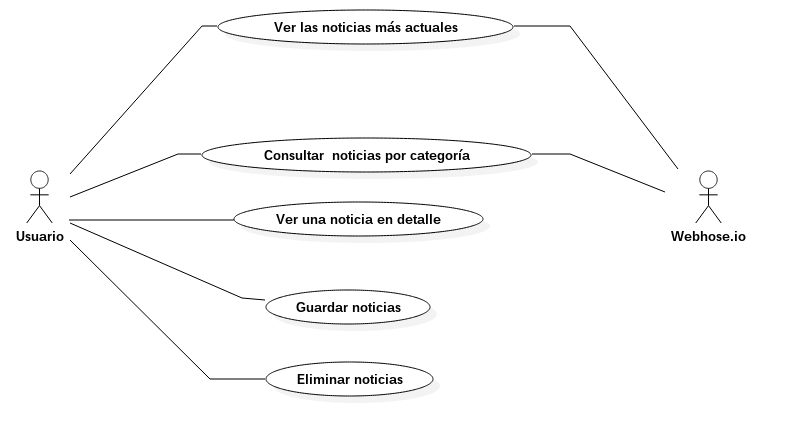
\includegraphics[scale=0.3,type=png,ext=.png,read=.png,angle=0,origin=c]{../diagramas/CU/runrunes/runrunesCU}
  \caption*{Diagrama de casos de uso definitivo de la aplicación Noticias+}
\end{figure}

\end{frame}



%----------------------------------------------------------------------------------------


\begin{frame}[fragile]
\frametitle{Eventos+}
\begin{figure}[H]
  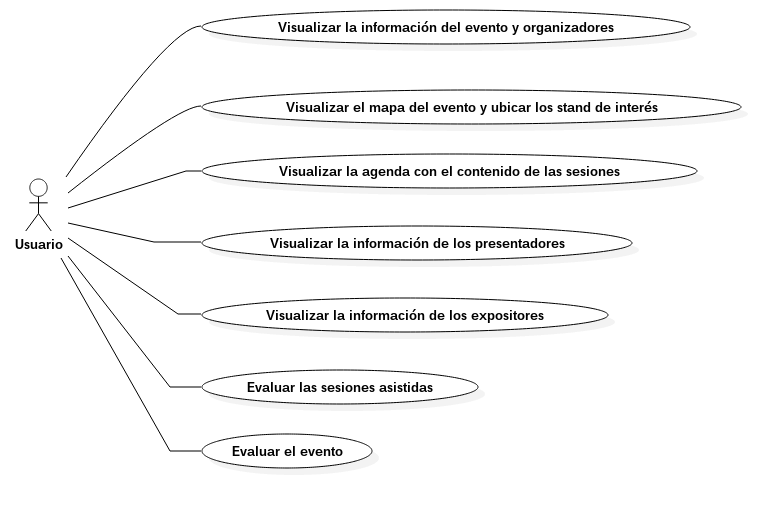
\includegraphics[scale=0.3,type=png,ext=.png,read=.png,angle=0,origin=c]{../diagramas/CU/eventos+/eventosCU}
  \caption*{Diagrama de casos de uso definitivo de la aplicación Eventos+}
\end{figure}

\end{frame}



%----------------------------------------------------------------------------------------





\begin{frame}[fragile]
\frametitle{Banca+ Móvil}
\begin{figure}[H]
  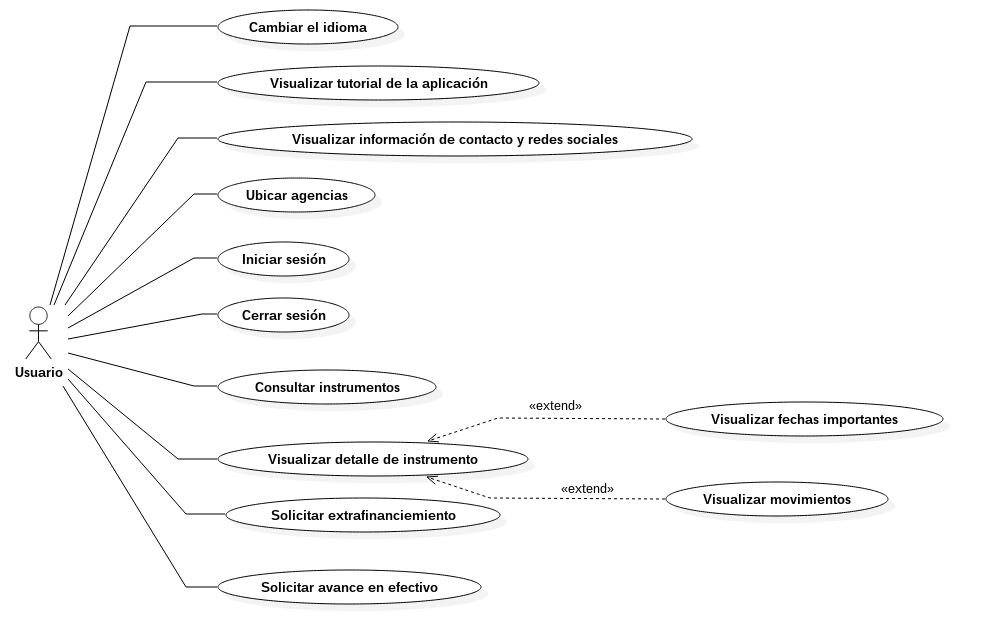
\includegraphics[scale=0.3,type=png,ext=.png,read=.png,angle=0,origin=c]{../diagramas/CU/banca+/bancaCU}
  \caption*{Diagrama de casos de uso parcial de la aplicación Banca+ Móvil}
\end{figure}

\end{frame}

%----------------------------------------------------------------------------------------

\begin{frame}[fragile]
\frametitle{Digitel}
\begin{figure}[H]
  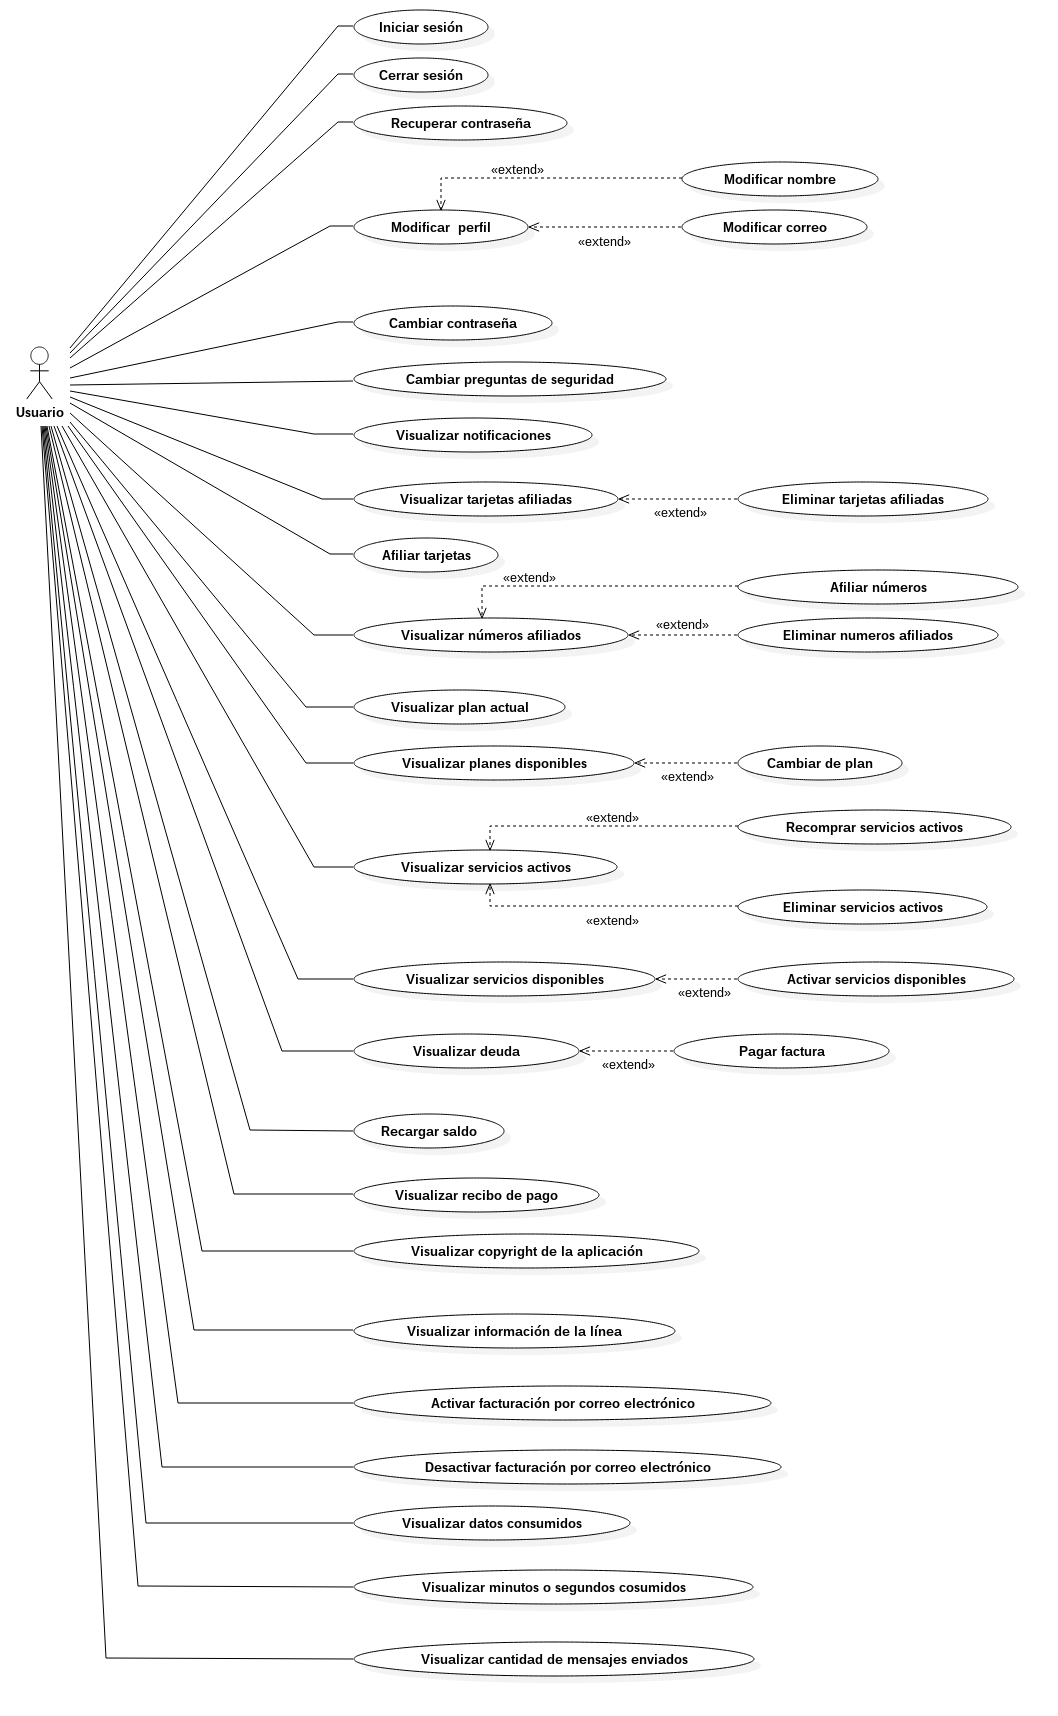
\includegraphics[scale=0.1,type=png,ext=.png,read=.png,angle=0,origin=c]{../diagramas/CU/digitel/digitelCU}
  \caption*{Diagrama de casos de uso definitivo de la aplicación Digitel}
\end{figure}

\end{frame}


%----------------------------------------------------------------------------------------
\subsection{Construcción}

\begin{frame}[fragile]
\frametitle{Construcción}
\begin{itemize}
	\item Noticias+
	\item Eventos+
	\item Digitel
	\item Banca+ Móvil
\end{itemize}

\end{frame}

%-------------------------------------------

\begin{frame}[fragile]
\frametitle{Noticias+}
\begin{itemize}
	\item Características:
	\begin{itemize}
		\item API Público: webhose.io
		\item Persistencia de datos
	\end{itemize}
\end{itemize}
     
\textbf{\href{videos/demo-noticias.mp4}{$\rightarrow$ Demo}} 

\end{frame}

%\begin{frame}[fragile]
%\frametitle{Noticias+}
%\begin{figure}[H]
 % \includegraphics[scale=0.3,type=png,ext=.png,read=.png,angle=0,origin=c]%{../imagenes/noticias}
  %\caption*{Mapa de navegación de la aplicación Noticias+}
%\end{figure}

%\end{frame}

%---------------------------------------------



\begin{frame}[fragile]
\frametitle{Eventos+}
%\begin{figure}[H]
%  \includegraphics[scale=0.3,type=png,ext=.png,read=.png,angle=0,origin=c]{../imagenes/eventos}
%  \caption*{Mapa de navegación de la aplicación Eventos+}
%\end{figure}


\textbf{ \href{videos/demo-eventos.mp4}{$\rightarrow$ Demo}}


\end{frame}


%---------------------------------------------

\begin{frame}[fragile]
\frametitle{Digitel}
\begin{itemize}
	\item Características:
	\begin{itemize}
		\item Cinco módulos bien definidos
		\item Integración total con una capa de servicios REST
	\end{itemize}
	\item Retos o problemas encontrados durante el desarrollo: 
	\begin{itemize}
		\item Navegación tipo slide ineficiente
		\item Manejo de la expiración de sesión
	\end{itemize}
\end{itemize}


\textbf{\href{videos/demo-digitel.mp4}{$\rightarrow$ Demo}} 



\end{frame}

%\begin{frame}[fragile]
%\frametitle{Digitel}
%\begin{figure}[H]
%  \includegraphics[scale=0.18,type=png,ext=.png,read=.png,angle=0,origin=c]{../imagenes/digitel1}
%  \caption*{Mapa de navegación de los módulos de autenticación, dashboard y pago de
%Digitel}
%\end{figure}

%\end{frame}

%\begin{frame}[fragile]
%\frametitle{Digitel}
%\begin{figure}[H]
 % \includegraphics[scale=0.27,type=png,ext=.png,read=.png,angle=0,origin=c]{../imagenes/digitel2}
  %\caption*{Mapa de navegación del módulo de menú de Digitel}
%\end{figure}

%\end{frame}

%---------------------------------------------

\begin{frame}[fragile]
\frametitle{Banca+ Móvil}
\begin{itemize}
	\item Características:
	\begin{itemize}
		\item Diseño en base a plantillas
		\item Estilo(CSS) parametrizado
	\end{itemize}
	\item Retos o problemas encontrados durante el desarrollo: 
	\begin{itemize}
		\item Manejo de la extensión y expiración de sesión
	\end{itemize}
\end{itemize}

\textbf{\href{videos/demo-banca.mp4}{$\rightarrow$ Demo}}


\end{frame}

%\begin{frame}[fragile]
%\frametitle{Banca+ Móvil}
%\begin{figure}[H]
 % \includegraphics[scale=0.22,type=png,ext=.png,read=.png,angle=0,origin=c]{../imagenes/banca}
 % \caption*{Mapa de navegación de Banca+ Móvil}
%\end{figure}
%\end{frame}

%---------------------------------------------

\subsection{Transición}

\begin{frame}[fragile]
\frametitle{Transición}
\begin{itemize}
	\item Esta fase solo fué llevada a cabo en la aplicación de Digitel debido a que la fecha de salida a producción era próxima al periodo de finalización de la pasantía
	\begin{itemize}
		\item Se realizaron un total de 184 Pruebas
		\item La aplicación salió al mercado el 22 de enero del 2016 para Android
	\end{itemize}
\end{itemize}

\end{frame}

%---------------------------------

\section{Conclusiones y Recomendaciones}

\begin{frame}[fragile]
\frametitle{Conclusiones y Recomendaciones}
\begin{itemize}
\item Conclusiones
	\begin{itemize}
		\item Aplicaciones nativas vs Aplicaciones Híbridas
		\item Un framework como forma de trabajo
	\end{itemize}
\item Recomendaciones
	\begin{itemize}
		\item Continuar el desarrollo de Kiraso
		\item Establecer el alcance del framework y de los componentes
		\item Seguir la línea de desarrollo del producto Banca+ Móvil
		\item Pruebas de calidad automatizadas
	\end{itemize}
\end{itemize}
\end{frame}

%-----------------------------------------------

\begin{frame}
\Huge{\centerline{¿Preguntas?}}
\end{frame}


%----------------------------------------------------------------------------------------

\section{Bibliografía}

\begin{frame}
        \frametitle{Bibliografía}        
        \begin{thebibliography}{99}

  		\bibitem[1]{MTFW1}
  			\emph{Where do frameworks fit in application development?},
  			http://www.lansa.com/resources/where-do-frameworks-fit-in-application-development.html,
  			consultado el 8 de enero de 2016
  			
    		\bibitem[2]{MTMD}
    			Rebecca Guenther; Jacqueline Radebaugh,
  			\emph{Understanding Metadata},
  			http://www.lansa.com/resources/where-do-frameworks-fit-in-application-development.html,
  			NISO Press, 2004
  			



		\end{thebibliography}
\end{frame}


\end{document} 